\documentclass[crop,tikz]{standalone}
\usepackage{makeidx,fancybox,tikz,nicematrix}
\usetikzlibrary{automata, graphs,positioning, arrows,patterns,shapes.geometric,shapes.multipart,shapes.symbols,shapes.arrows}
\usetikzlibrary{arrows.meta}

%\usegdlibrary{trees,layered}
\pgfdeclarelayer{background}
\pgfdeclarelayer{foreground}
\pgfsetlayers{background,main,foreground}

\usetikzlibrary{fit, calc}
\usepackage{xparse}
\makeatletter
\NewDocumentCommand {\getnodedimen} {O{\nodewidth} O{\nodeheight} m} {
  \begin{pgfinterruptboundingbox}
  \begin{scope}[local bounding box=bb@temp]
    \node[inner sep=0pt, fit=(#3)] {};
  \end{scope}
  \path ($(bb@temp.north east)-(bb@temp.south west)$);
  \end{pgfinterruptboundingbox}
  \pgfgetlastxy{#1}{#2}
}
\makeatother

\begin{document}


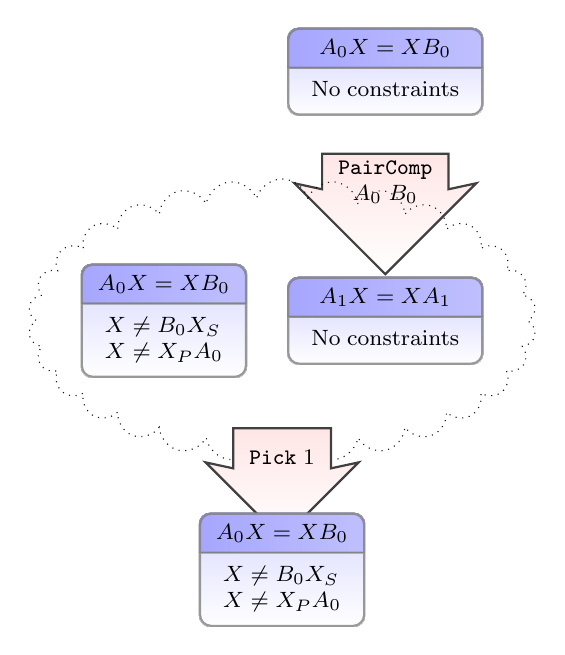
\begin{tikzpicture}[
level 0/.style = {sibling distance = 8em,level distance = 3em},
level 0/.style = {sibling distance = 8em,level distance = 2em},
level 1/.style = {sibling distance = 6em,level distance = 4em},
level 2/.style = {sibling distance = 8em,level distance = 5em},
level 3/.style = {sibling distance = 6em,level distance = 5em},
level 4/.style = {sibling distance = 8em,level distance = 4em},
]


\tikzstyle{equation}=[rectangle, draw opacity=0.8,rounded corners,thick,draw=black!75,top color=blue!10, bottom color=white,minimum size=5mm, font =\footnotesize]
\tikzstyle{eqset}=[draw,cloud,dotted,opacity=0.9]
\tikzstyle{failequation}=[rectangle split,rectangle split parts=2,
    rounded corners,
    thick,
    draw=black!50,
    draw opacity=0.8,
    minimum size=5mm, font =\footnotesize
    ,append after command={\pgfextra
        \fill[left color=red!35!gray, right color=red!55!gray]
    (\tikzlastnode.one west) 
    [rounded corners] |- (\tikzlastnode.north) -| (\tikzlastnode.one east) 
    [sharp corners]   |- (\tikzlastnode.one split) -| cycle;
        \fill[top color=gray!15, bottom color=white]
    (\tikzlastnode.two west) 
    [rounded corners] |- (\tikzlastnode.south) -| (\tikzlastnode.two east)  
    [sharp corners]   |- (\tikzlastnode.one split) -| cycle;
                                    \endpgfextra}]
\tikzstyle{fullequation}=[rectangle split,rectangle split parts=2,
    rounded corners,
    thick,
    draw=black!50,
    draw opacity=0.8,
    minimum size=5mm, font =\footnotesize
    ,append after command={\pgfextra
        \fill[left color=blue!35, right color=blue!25]
    (\tikzlastnode.one west) 
    [rounded corners] |- (\tikzlastnode.north) -| (\tikzlastnode.one east) 
    [sharp corners]   |- (\tikzlastnode.one split) -| cycle;
        \fill[top color=blue!10, bottom color=white]
    (\tikzlastnode.two west) 
    [rounded corners] |- (\tikzlastnode.south) -| (\tikzlastnode.two east)  
    [sharp corners]   |- (\tikzlastnode.one split) -| cycle;
                                    \endpgfextra}]
\tikzstyle{chosenequation}=[rectangle split,rectangle split parts=2,
    rounded corners,
    thick,
    double, double distance=1.5pt,
    draw=black!50,
    draw opacity=0.8,
    minimum size=5mm, font =\footnotesize
    ,append after command={\pgfextra
        \fill[left color=yellow!50, right color=yellow!35]
    (\tikzlastnode.one west) 
    [rounded corners] |- (\tikzlastnode.north) -| (\tikzlastnode.one east) 
    [sharp corners]   |- (\tikzlastnode.one split) -| cycle;
        \fill[top color=yellow!20, bottom color=white]
    (\tikzlastnode.two west) 
    [rounded corners] |- (\tikzlastnode.south) -| (\tikzlastnode.two east)  
    [sharp corners]   |- (\tikzlastnode.one split) -| cycle;
                                    \endpgfextra}]
\tikzstyle{action}=[single arrow,shape border rotate=270,inner sep=0.1ex,thick,draw=black!75,top color=red!10, bottom color=white,minimum height=4em,single arrow head extend=1em,single arrow head indent=0.5ex, font =\footnotesize,,opacity=1]
\tikzstyle{subst}=[shape aspect=4,diamond, thick,draw=black!75, top color=green!5, bottom color=white,minimum size=5mm] 

\node (0B0) [fullequation]{\nodepart{one}$A_{0}X = XB_{0}$\nodepart{two}$\begin{array}{l}\mathrm{No\;constraints}\\\end{array}$}
child {node [action]{$\begin{array}{c}\mathtt{PairComp}\\A_{0}\;B_{0}\end{array}$} edge from parent [draw opacity = 0]
child {node (2B0) [fullequation]{\nodepart{one}$A_{0}X = XB_{0}$\nodepart{two}$\begin{array}{l}X\neq{}B_{0}X_{S}\\X\neq{}X_{P}A_{0}\end{array}$}edge from parent [draw opacity = 0]
}
child {node (2B1) [fullequation]{\nodepart{one}$A_{1}X = XA_{1}$\nodepart{two}$\begin{array}{l}\mathrm{No\;constraints}\\\end{array}$}edge from parent [draw opacity = 0]
}
child {node [eqset,inner sep=-1em,cloud puffs=30,aspect=2,fit=(2B0)(2B1)] {}
child {node [action]{$\begin{array}{c}\mathtt{Pick}\;1\end{array}$} edge from parent [draw opacity = 0]
child {node (4B0) [fullequation]{\nodepart{one}$A_{0}X = XB_{0}$\nodepart{two}$\begin{array}{l}X\neq{}B_{0}X_{S}\\X\neq{}X_{P}A_{0}\end{array}$}edge from parent [draw opacity = 0]};};};};
\end{tikzpicture}

\end{document}
